%% 
%% Copyright 2007-2020 Elsevier Ltd
%% 
%% This file is part of the 'Elsarticle Bundle'.
%% ---------------------------------------------
%% 
%% It may be distributed under the conditions of the LaTeX Project Public
%% License, either version 1.2 of this license or (at your option) any
%% later version.  The latest version of this license is in
%%    http://www.latex-project.org/lppl.txt
%% and version 1.2 or later is part of all distributions of LaTeX
%% version 1999/12/01 or later.
%% 
%% The list of all files belonging to the 'Elsarticle Bundle' is
%% given in the file `manifest.txt'.
%% 

%% Template article for Elsevier's document class `elsarticle'
%% with numbered style bibliographic references
%% SP 2008/03/01
%%
%% 
%%
%% $Id: elsarticle-template-num.tex 190 2020-11-23 11:12:32Z rishi $
%%
%%
\documentclass[preprint,12pt]{elsarticle}

%% Use the option review to obtain double line spacing
%% \documentclass[authoryear,preprint,review,12pt]{elsarticle}

%% Use the options 1p,twocolumn; 3p; 3p,twocolumn; 5p; or 5p,twocolumn
%% for a journal layout:
%% \documentclass[final,1p,times]{elsarticle}
%% \documentclass[final,1p,times,twocolumn]{elsarticle}
%% \documentclass[final,3p,times]{elsarticle}
%% \documentclass[final,3p,times,twocolumn]{elsarticle}
%% \documentclass[final,5p,times]{elsarticle}
%% \documentclass[final,5p,times,twocolumn]{elsarticle}

%% For including figures, graphicx.sty has been loaded in
%% elsarticle.cls. If you prefer to use the old commands
%% please give \usepackage{epsfig}

%% The amssymb package provides various useful mathematical symbols
\usepackage{amssymb}
\usepackage{amsmath, bm}
%% The amsthm package provides extended theorem environments
%% \usepackage{amsthm}

%% The lineno packages adds line numbers. Start line numbering with
%% \begin{linenumbers}, end it with \end{linenumbers}. Or switch it on
%% for the whole article with \linenumbers.
%% \usepackage{lineno}
\usepackage{easyReview}
\usepackage{savesym}
\savesymbol{comment}

\usepackage{cases}
\restoresymbol{Review}{comment}

\usepackage{color}
\newcommand{\pt}[1]{{\color{red}{#1}}}
\newcommand{\ad}[1]{{\color{blue}{#1}}}
\newcommand{\de}[1]{{\color{gray}{#1}}}

\usepackage{todonotes}

\usepackage{hyperref}

\hypersetup{
	colorlinks=true,
	%	linkcolor=blue,
	filecolor=magenta,      
	urlcolor=cyan,
	pdftitle={Overleaf Example},
	pdfpagemode=FullScreen,
}

\usepackage{graphicx}
\usepackage{subfigure}
\usepackage{booktabs}

\usepackage{float}
\journal{NEURAL NETWORKS}


\setlength{\abovecaptionskip}{0.1cm}
\begin{document}
\setreviewson
\begin{frontmatter}

%% Title, authors and addresses

%% use the tnoteref command within \title for footnotes;
%% use the tnotetext command for theassociated footnote;
%% use the fnref command within \author or \address for footnotes;
%% use the fntext command for theassociated footnote;
%% use the corref command within \author for corresponding author footnotes;
%% use the cortext command for theassociated footnote;
%% use the ead command for the email address,
%% and the form \ead[url] for the home page:
%% \title{Title\tnoteref{label1}}
%% \tnotetext[label1]{}
%% \author{Name\corref{cor1}\fnref{label2}}
%% \ead{email address}
%% \ead[url]{home page}
%% \fntext[label2]{}
%% \cortext[cor1]{}
%% \affiliation{organization={},
%%             addressline={},
%%             city={},
%%             postcode={},
%%             state={},
%%             country={}}
%% \fntext[label3]{}

\title{PhaseCANN: An continuous attractors neural network model for grid-cell module.}

%% use optional labels to link authors explicitly to addresses:
%% \author[label1,label2]{}
%% \affiliation[label1]{organization={},
%%             addressline={},
%%             city={},
%%             postcode={},
%%             state={},
%%             country={}}
%%
%% \affiliation[label2]{organization={},
%%             addressline={},
%%             city={},
%%             postcode={},
%%             state={},
%%             country={}}

\author[a,b,c]{Zhihui Zhang}
\author[b,c]{Fengzhen Tang}
\author[b,c]{Yiping Li}
\author[b,c]{Xisheng Feng}
\affiliation[a]{organization={University of Science and technology of China},%Department and Organization
            addressline={No.96, JinZhai Road Baohe District}, 
            city={Hefei},
            postcode={230026}, 
            state={Anhui},
            country={China}}
\affiliation[b]{organization={The State Key Laboratory of Robotics, Shenyang
			Institute of Automation, Chinese Academy of Science},%Department and Organization
            addressline={No.135, Chuangxin Road Hunnan District}, 
            city={Shenyang},
            postcode={110016}, 
            state={Liaoning},
            country={China}}
\affiliation[c]{organization={Institutes for Robotics and Intelligent Manufacturing, Chinese Academy of Sciences},%Department and Organization
            addressline={No.135, Chuangxin Road Hunnan District}, 
            city={Shenyang},
            postcode={110169}, 
            state={Liaoning},
            country={China}}
            
\begin{abstract}
Although grid cells in the entorhinal cortex are regarded to be a key component of spatial cognition in animals, the latent mechanisms of grid-cell firing are still up for discussion. Current computational models focus more on the activity of single grid cells. However, It has been found that the grid-cell activity was generally organized into a small number of discrete functional modules\cite{Stensola2012}. Here, we proposed a continuous attractors network(CAN) model for grid-cell modules. Our model is driven using self-motion inputs and injected energy by external cues. The neurons in the CAN can present the hexagonal firing patterns with driving the model for grid-cell modules. Our model simultaneously shows the path integration capability that a grid-cell module is thought to have. Even when lacks external cues, our model predicts the prominent performance of path integration for grid-cell modules over long distances.

\end{abstract}

% %%Graphical abstract
% \begin{graphicalabstract}
% \includegraphics{grabs}
% \end{graphicalabstract}

% %%Research highlights
% \begin{highlights}
% \item Research highlight 1
% \item Research highlight 2
% \end{highlights}

\begin{keyword}
%% keywords here, in the form: keyword \sep keyword
Grid cell \sep Place cell  \sep Continuous attractors network \sep Path integration
%% PACS codes here, in the form: \PACS code \sep code
%\PACS 0000 \sep 1111
%%% MSC codes here, in the form: \MSC code \sep code
%%% or \MSC[2008] code \sep code (2000 is the default)
%\MSC 0000 \sep 1111
\end{keyword}

\end{frontmatter}

%% \linenumbers

%% main text
\section{Introduction}
The grid cells are important neurons that are discovered in the medial entorhinal cortex(mEC)\cite{Moser2017}. The grid cells have hexagonally arranged firing fields that can cover entire environment that a freely moving animal has passed through\cite{Rowland2016}. In addition, the grid cells have found in many kind of animals, including rat, mice\cite{Fyhn2008}, bats\cite{Yartsev2011}, monkey\cite{Killian2012} and human\cite{Jacobs2013,Kunz2015,Doeller2010}. This shows that the grid cells widely exist in mEC as an important role in the cognitive map of rodent animals. Since the discovery of the grid cells, the function of them in cognitive map keep drawing attention to researchers all the time. Although so, the latent mechanisms how to form the grid-like patterns still remain a mystery\cite{DAlbis2017}.


Oscillatory-interference(OI) models of grid cells are proposed in the early 1990s to explain the origin of place field and their relationship with the hippocampal theta rththm\cite{OKeefe2005,Burgess2007,Hasselmo2007,Pastoll2013,Burgess2008}. The dual-oscillator model can explain the emergence of place fields and phase procession\cite{OKeefe2005}. At the same time, it also can intrinsically generate periodic patterns. So it was used to try to explain the periodic firing fields of grid cells\cite{DAlbis2018}. In this models, the periodic patterns are generated by interfering with multiple oscillators that have different frequencies. These oscillators with different frequencies are modulated by the moving speed and direction of the animals. So such oscillators are called velocity-controlled oscillators(VCO). By this, only two VCOs are enough to generate grid-like patterns. 
Although the OI models have been supported by some researches\cite{Schmidt-Hieber2013,Domnisoru2013,Welday2011,Koenig2011,Brandon2011,Giocomo2007,Hafting2005,Alonso1989}, there are still some problem for OI theory. An problem of OI models is the 60 degree angle between multiple VCOs needs to be specified manually. Additionally, The grid-like patterns of OI models can be rapidly disrupted by noise\cite{DAlbis2018}.


The CANN models are a type of very influential model in the field of computational neuroscience. The fundamental premise of such models is that a correctly designed recurrent network may sustain a continuous stable states in its neurons activity\cite{Taylor1999,Amari1977}. Multiple CANN models of grid cells have been proposed to explain the grid-like patterns\cite{Fuhs2006,Burak2009,Guanella2007,Shipston-Sharman2016,Couey2013}. In these models, there are multiple bumps of activity in the CANN of grid cells by the weight profile of Mexican-hat or Lincoln-hat\cite{Rowland2016}. Then the bumps in networks can be driven by self-motion cues. Rodents can utilize self-motion cues to navigate across short distances, which is consistent with the feature of the CANN. And CANN have been witnessed to be in line with the modular organization of grid cell activity\cite{Stensola2012,Yoon2013}. Nevertheless, these are some weakness in CAN models. The CANN models require a complex neural network architecture. But this architecture has an unknown development genesis. Additionally, they require anchoring to the physical and are unable to describe how environmental geometry and sensory input alter grid fields\cite{DAlbis2017}.

Although many models mentioned above have been proposed to explain the grid-like firing field of grid cells, the latent mechanism of grid cells still be vague. For every kind of models, there is some supported and against evidence. The CANN models have been widely applied to multiple recognized cells in the entorhinal–hippocampal neuronal circuits, such as head direction cells and place cells. In addition, the CANN models is naturally suitable to process the path integration in cognitive map. So in the research area of cognitive map and robot navigation, the CANN models acquire more attention. However, current CANN models of grid cells try to take consideration all properties of grid cells. This make current models have some obvious artifacts. For example, In \cite{Guanella2007}, the neurons in CANN are manually organized in a plane covering the repetitive rectangular structure to generate the hexagonal firing patterns. Additionally, in \cite{Guanella2007}, the CANN models of grid cells receive the input from the CANN models of place cells connecting by the Hebbian rules. But this can not make the CANN models of grid cells anchor to the physical world\cite{DAlbis2017}.

In addition, current models focus more on single grid-cell activity. But grid-cell activity was discovered to be usually structured into a small number of distinct functional modules. So in here, we focus on a grid-cell module and proposed a new CANN models for the grid-cell module. Because in a single module, all grid cells have same spacing and orientation\cite{Stensola2012}. So in our model of grid cells, the neurons that represented grid cells are arranged in a plane according to their own phases. So our CANN model is marked as PhaseCANN. In this way, the structure of the PhaseCANN is established like the CANN models of place cells\cite{McNaughton2006}. This improves the overall network structure's naturalness comparing with the CANN of grid-cell model\cite{Guanella2007}. In addition, we build a direct connection between place cell and grid-cell module using the spatial transformation. By this connection, the deviation of path integration can be corrected in the CANN model of grid cells based on phase. Then the single grid-cell activity, the activity of grid-cell module based on our model are recorded. They are consistent with the biological experiment about single grid-cell activity\cite{Hafting2005}. Finally, the performance of the path integration using our model is evaluated in different spacing, sizes of network, moving steps. The results demonstrate that our model performs very well across extended distances and without external cues.


\section{Results}

\subsection{The structure of proposed model}\label{subsection:structure}

\begin{figure*}[!t]
%	\subfigcapskip=-5pt %调整子图片与子标题的距离
	\centering
	\subfigure[]{
		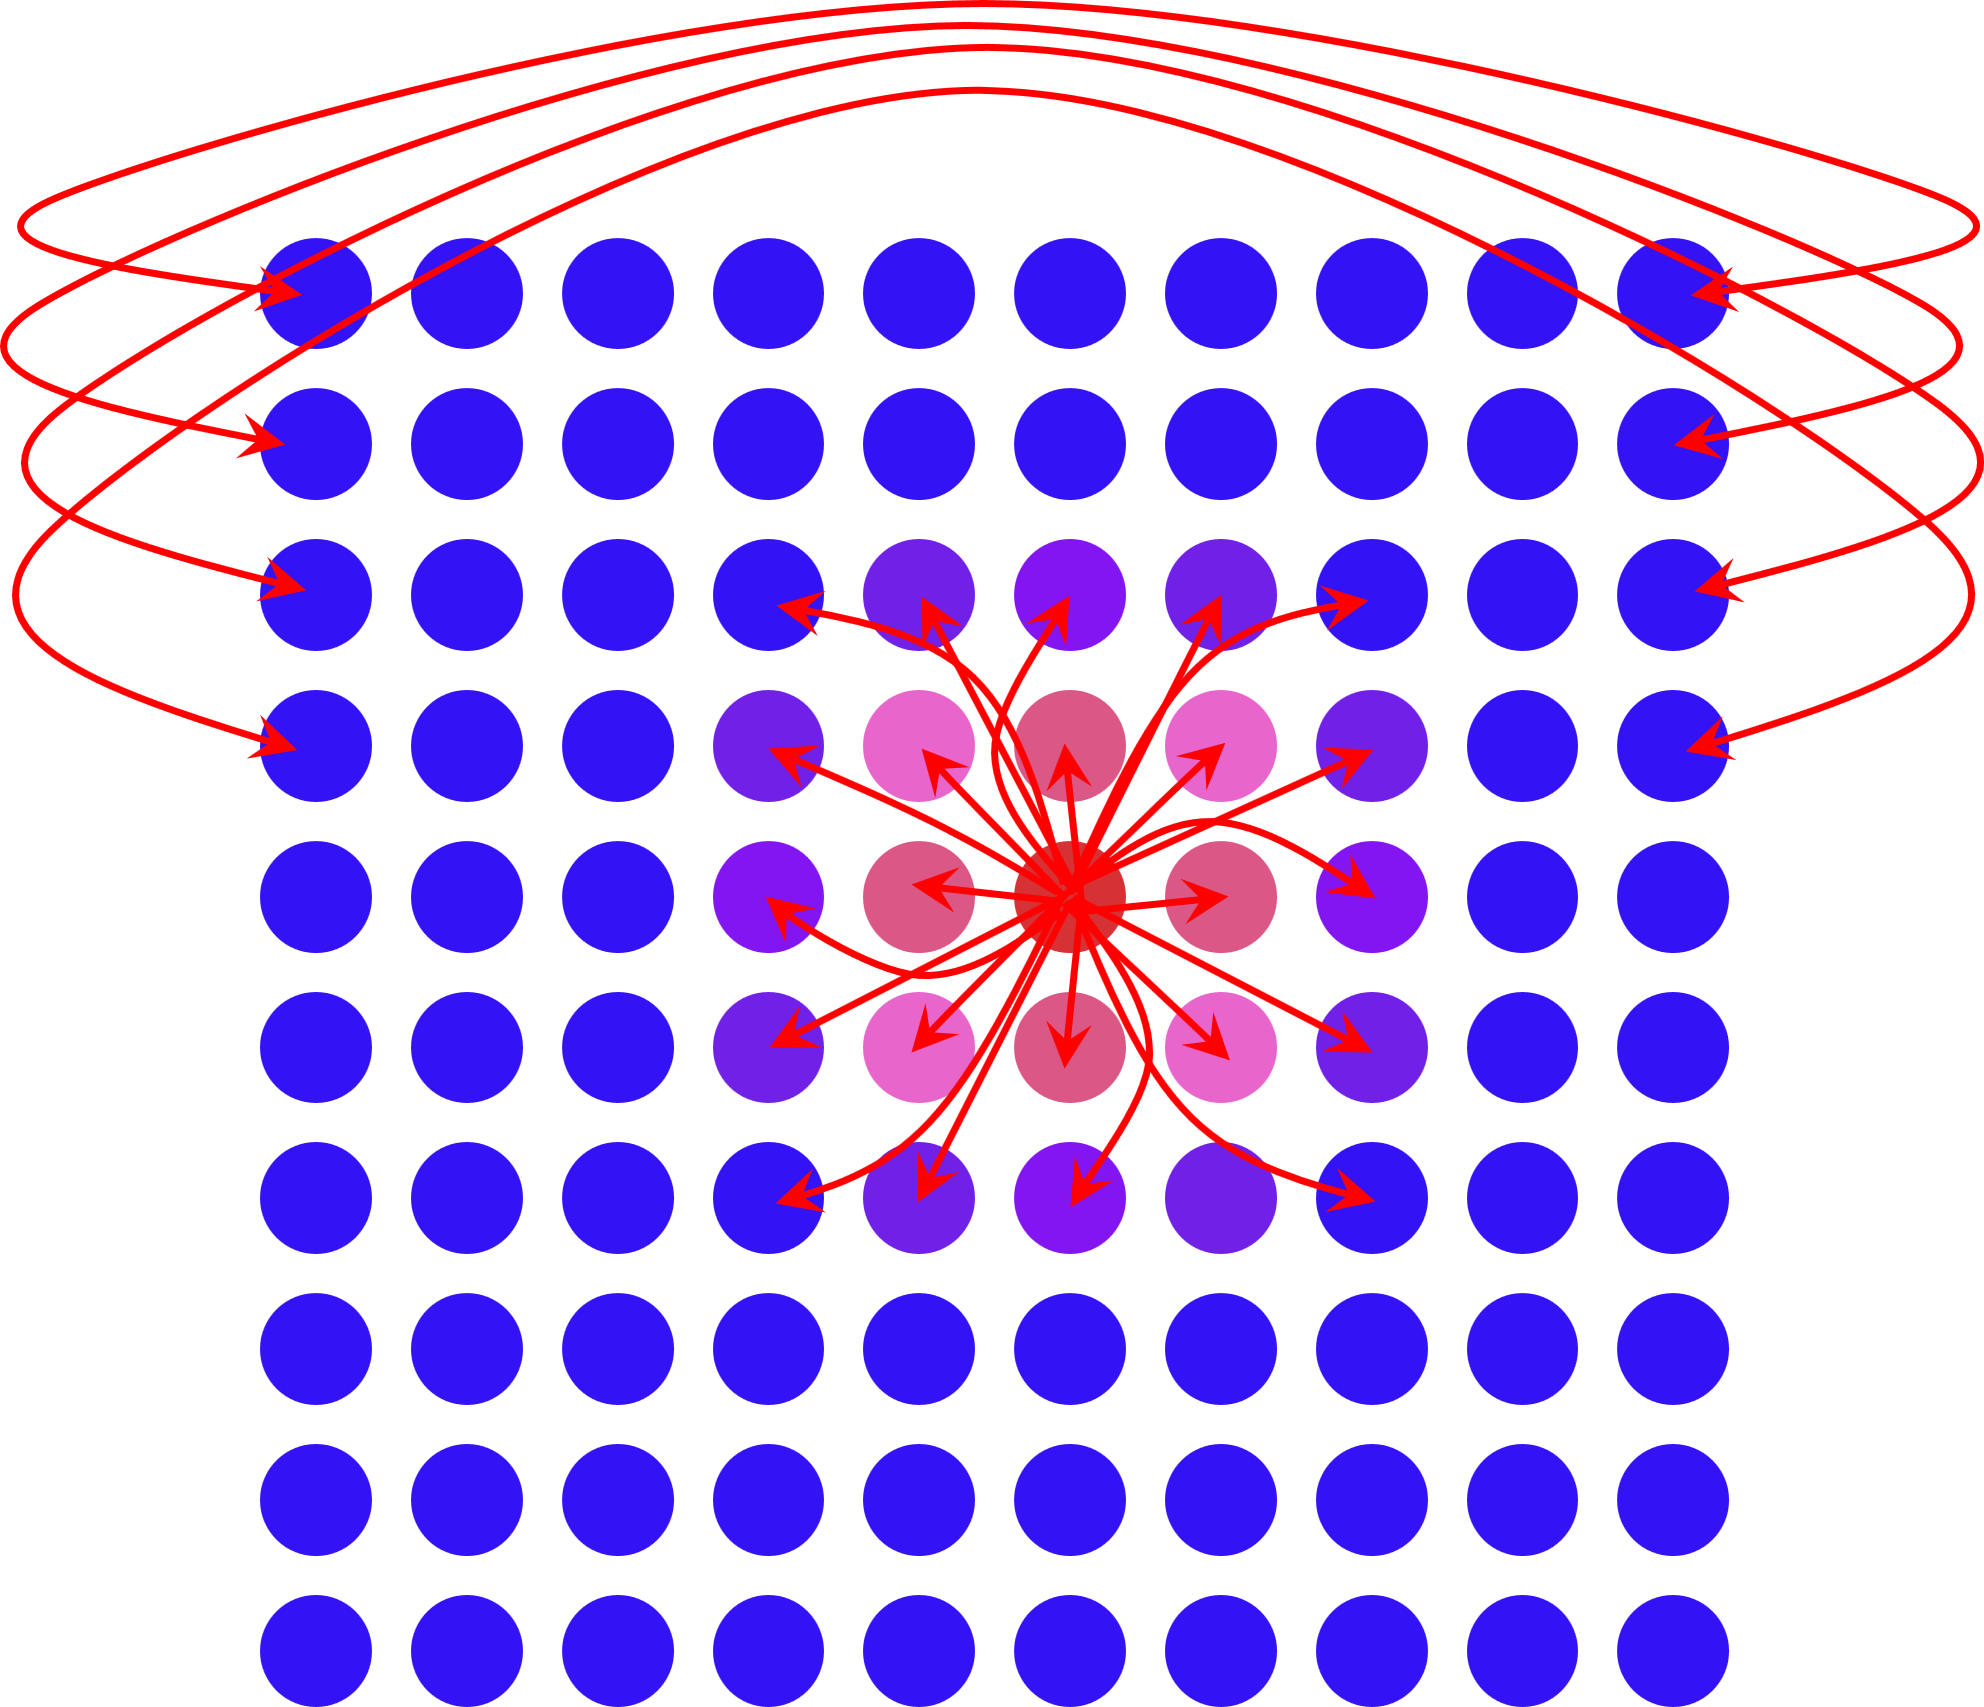
\includegraphics[width=0.45\linewidth]{Figure/2D_structure.png}
		%\caption{fig1}
		\label{fig:cann_structure_a}
	}
	\hspace{-2pt}	
	\subfigure[]{
		\includegraphics[width=0.45\linewidth]{Figure/3D_structure.png}
		\label{fig:cann_structure_b}
	}

	\caption{The phase cann structure}
	\label{fig:cann_structure}
\end{figure*}


In the reference \cite{Stensola2012}, it shows that grid cells form discrete modules. And each grid module shares a common spacing, orientation\cite{Rowland2016}. Previous models of grid cells more focus on explaining the firing patterns of a single grid cell. In here, we concentrate on single grid module and explore its firing mechanism. As Fig.~\ref{fig:cann_structure_a} depicted, in our model, the neurons of grid cells in same module are arranged in a sheet. In this sheet, the population neurons are defined as follows:
\begin{equation}
	M = N_x \times N_y
\end{equation}
where $N$ is the amount of the neurons of grid cells, $N_x$ is the amount of the neurons in the horizontal direction, $N_y$ is the amount of the neurons in the vertical direction. In our model, the relationship of $N_x$ and $N_y$ are defined by:
\begin{equation}\label{eq:network_size}
	N_x = N_y = N
\end{equation}


To simply demonstrate the proposed model, a grid cell can be represented as follows:
\begin{equation}
	\bm{G_i} = [s_i,o_i,\bm{\vartheta_i}],~i\in \bm{Z^+}
\end{equation}
where $s_i$ represents the spacing of the grid cell $\bm{G_i}$, $o_i$ represents the orientation of the grid cell $\bm{G_i}$, $\bm{\vartheta_i}$ represents the phase of the grid cell $\bm{G_i}$ and $\bm{\vartheta_i} = [\vartheta_i^1,\vartheta_i^2]$ contains the phases of the two directions.

For the grid cells in a module, they share common spacing and orientation. So the grid cells of the same module can be further represented as follows:
\begin{equation}
	\bm{G_i} = [s,o,\bm{\vartheta_i}], i\in \bm{Z^+}
\end{equation}

A grid cell $\bm{G_i}$ in a module can be placed in the sheet according to its phases. Different from the CANN model in the reference\cite{Guanella2007}, all neurons $\epsilon_{xy}$ in our model are arranged as a matrix instead of repetitive rectangular structure. According to the phases of the grid cell $\bm{G_i}$, the index $(x,y)$ of a neuron $\epsilon_{xy}$ in the matrix can be described as follows:

\begin{numcases}{}
	x = \frac{\vartheta_i^1}{\Delta \vartheta^1}\\
	y = \frac{\vartheta_i^2}{\Delta \vartheta^2}
\end{numcases}
where $\Delta \vartheta$ is the phase gap of neighbor neurons, $\vartheta_i^1$ and $\vartheta_i^2$ are the phases of $\bm{G_i}$. As Fig.~\ref{fig:cann_structure_a} depicted, the neurons in our model are connected recurrently and have the periodic boundary condition. So the max phase of the neurons in the model is equal to the spacing of the grid module. Then $\Delta \vartheta$ can be further calculated as follows:
\begin{equation}
	\Delta \vartheta = \frac{s}{N}
\end{equation}
where $s$ is the spacing of the grid-cell module, $N$ is the size of the CANN model.
\subsection{The connection of proposed model}\label{subsection:connection}
\begin{figure}[!t]
	\centering
	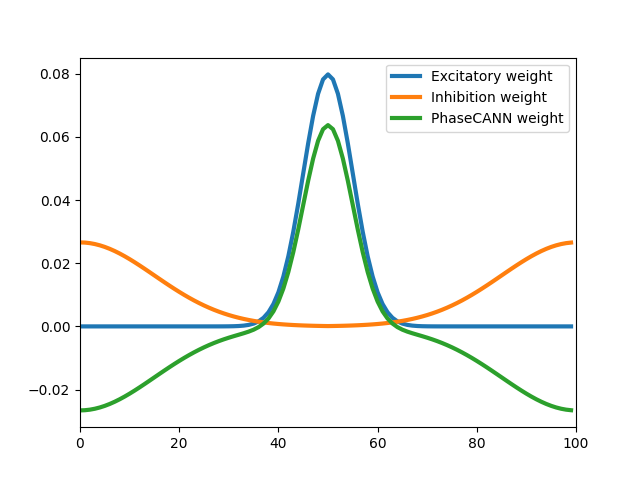
\includegraphics[width=0.8\linewidth]{Figure/weight_profile.png}
	\caption{The weight profile of the PhaseCANN. The weight profile of the PhaseCANN consists of two part. One part is the excitatory weight to activate the local neurons. The another part is the inhibition part and it inhibit distant neurons. The two part is used to compute the weight profile of the PhaseCANN by Eq.~\eqref{eq:weight_gc}. }	
	\label{fig:weight_profile}
\end{figure}
As mentioned above, the grid cells neurons in identical module are arranged in a sheet. They are connected with each other and have periodic boundary condition. This is depicted in Fig.~\ref{fig:cann_structure}. For these grid cells that have same spacing and orientation in identical module according to \cite{Burak2009}, the dynamic of rate-based neurons can be described by:
\begin{equation}\label{eq:firing_rate}
	\tau \frac{d r_{i}}{d t}+r_{i}=f\left[\sum_{j} w_{i j} r_{j}\right]
\end{equation}
where $\tau$ is the time-constant of neuron response, $r_i$ is spike rate of the neuron, $f$ is a non-linearity function and can be described as follows:
\begin{numcases}{f(x)=}
	=x, x>0\\ 
	=0, otherwise
\end{numcases}
	
The $w_{ij}$ in Eq.~\eqref{eq:firing_rate} is the connection weight from neurons $\epsilon_j$ and neuron $\epsilon_i$. It includes two parts. The first part is used to exciting the neighbor neurons of the neuron $\epsilon_j$. The second part is utilized to inhibit the neighbor neurons of the neuron $\epsilon_j$. In here, two Gaussian function are used to generate the weight profile. The weight is depicted in Fig.~\ref{fig:weight_profile}. So $w_{ij}$ can be described as follows:
\begin{equation}\label{eq:weight_gc}
	w_{ij}=\alpha e^{-\rho d_{ij}^2} - \beta e^{-\gamma (d_{ij}-D)^2}
\end{equation}
where $w_{ij}$ is the weight from $\epsilon_{j}$ to $\epsilon_{i}$, $\alpha,\rho,\beta,\gamma$ are the hyper-parameters to adjust the scope of Gaussian function, $D$ is the max distance of two neurons in the network, $d$ is the distance between $\epsilon_{j}$ and $\epsilon_{i}$ and it can be computed as follows:

\begin{align}
	d_{ij} &= ||\epsilon_{i} - \epsilon_{j}||_2 \\
	&=\sqrt{(x_i-x_j)^2+(y_i-y_j)^2}	 
\end{align}	

\subsection{Activity and stabilization}

Place cells have been considered to provided the input for grid cells. The experiment that recorded the neural activity in the medial entorhinal cortex(MEC) of rat after temporary inactivation of the hippocampus shows that grid cells will lost their grid-like firing patterns and tune to the direction of the rat's head\cite{Bonnevie2013}. To make gird cells acquire the input from the place cells, the CANN of place cells\cite{McNaughton2006} is used to inject the activity to the PhaseCANN. As depicted in Fig.~\ref{fig:w2p2g}, for a landmark in the true world, it can be mapping to a neuron activity in the place cell sheet. \alert{According to our previous work}, a landmark $P^w_i$ was firstly transformed into place cell firing space by:

\begin{figure*}[!t]
	\centering
	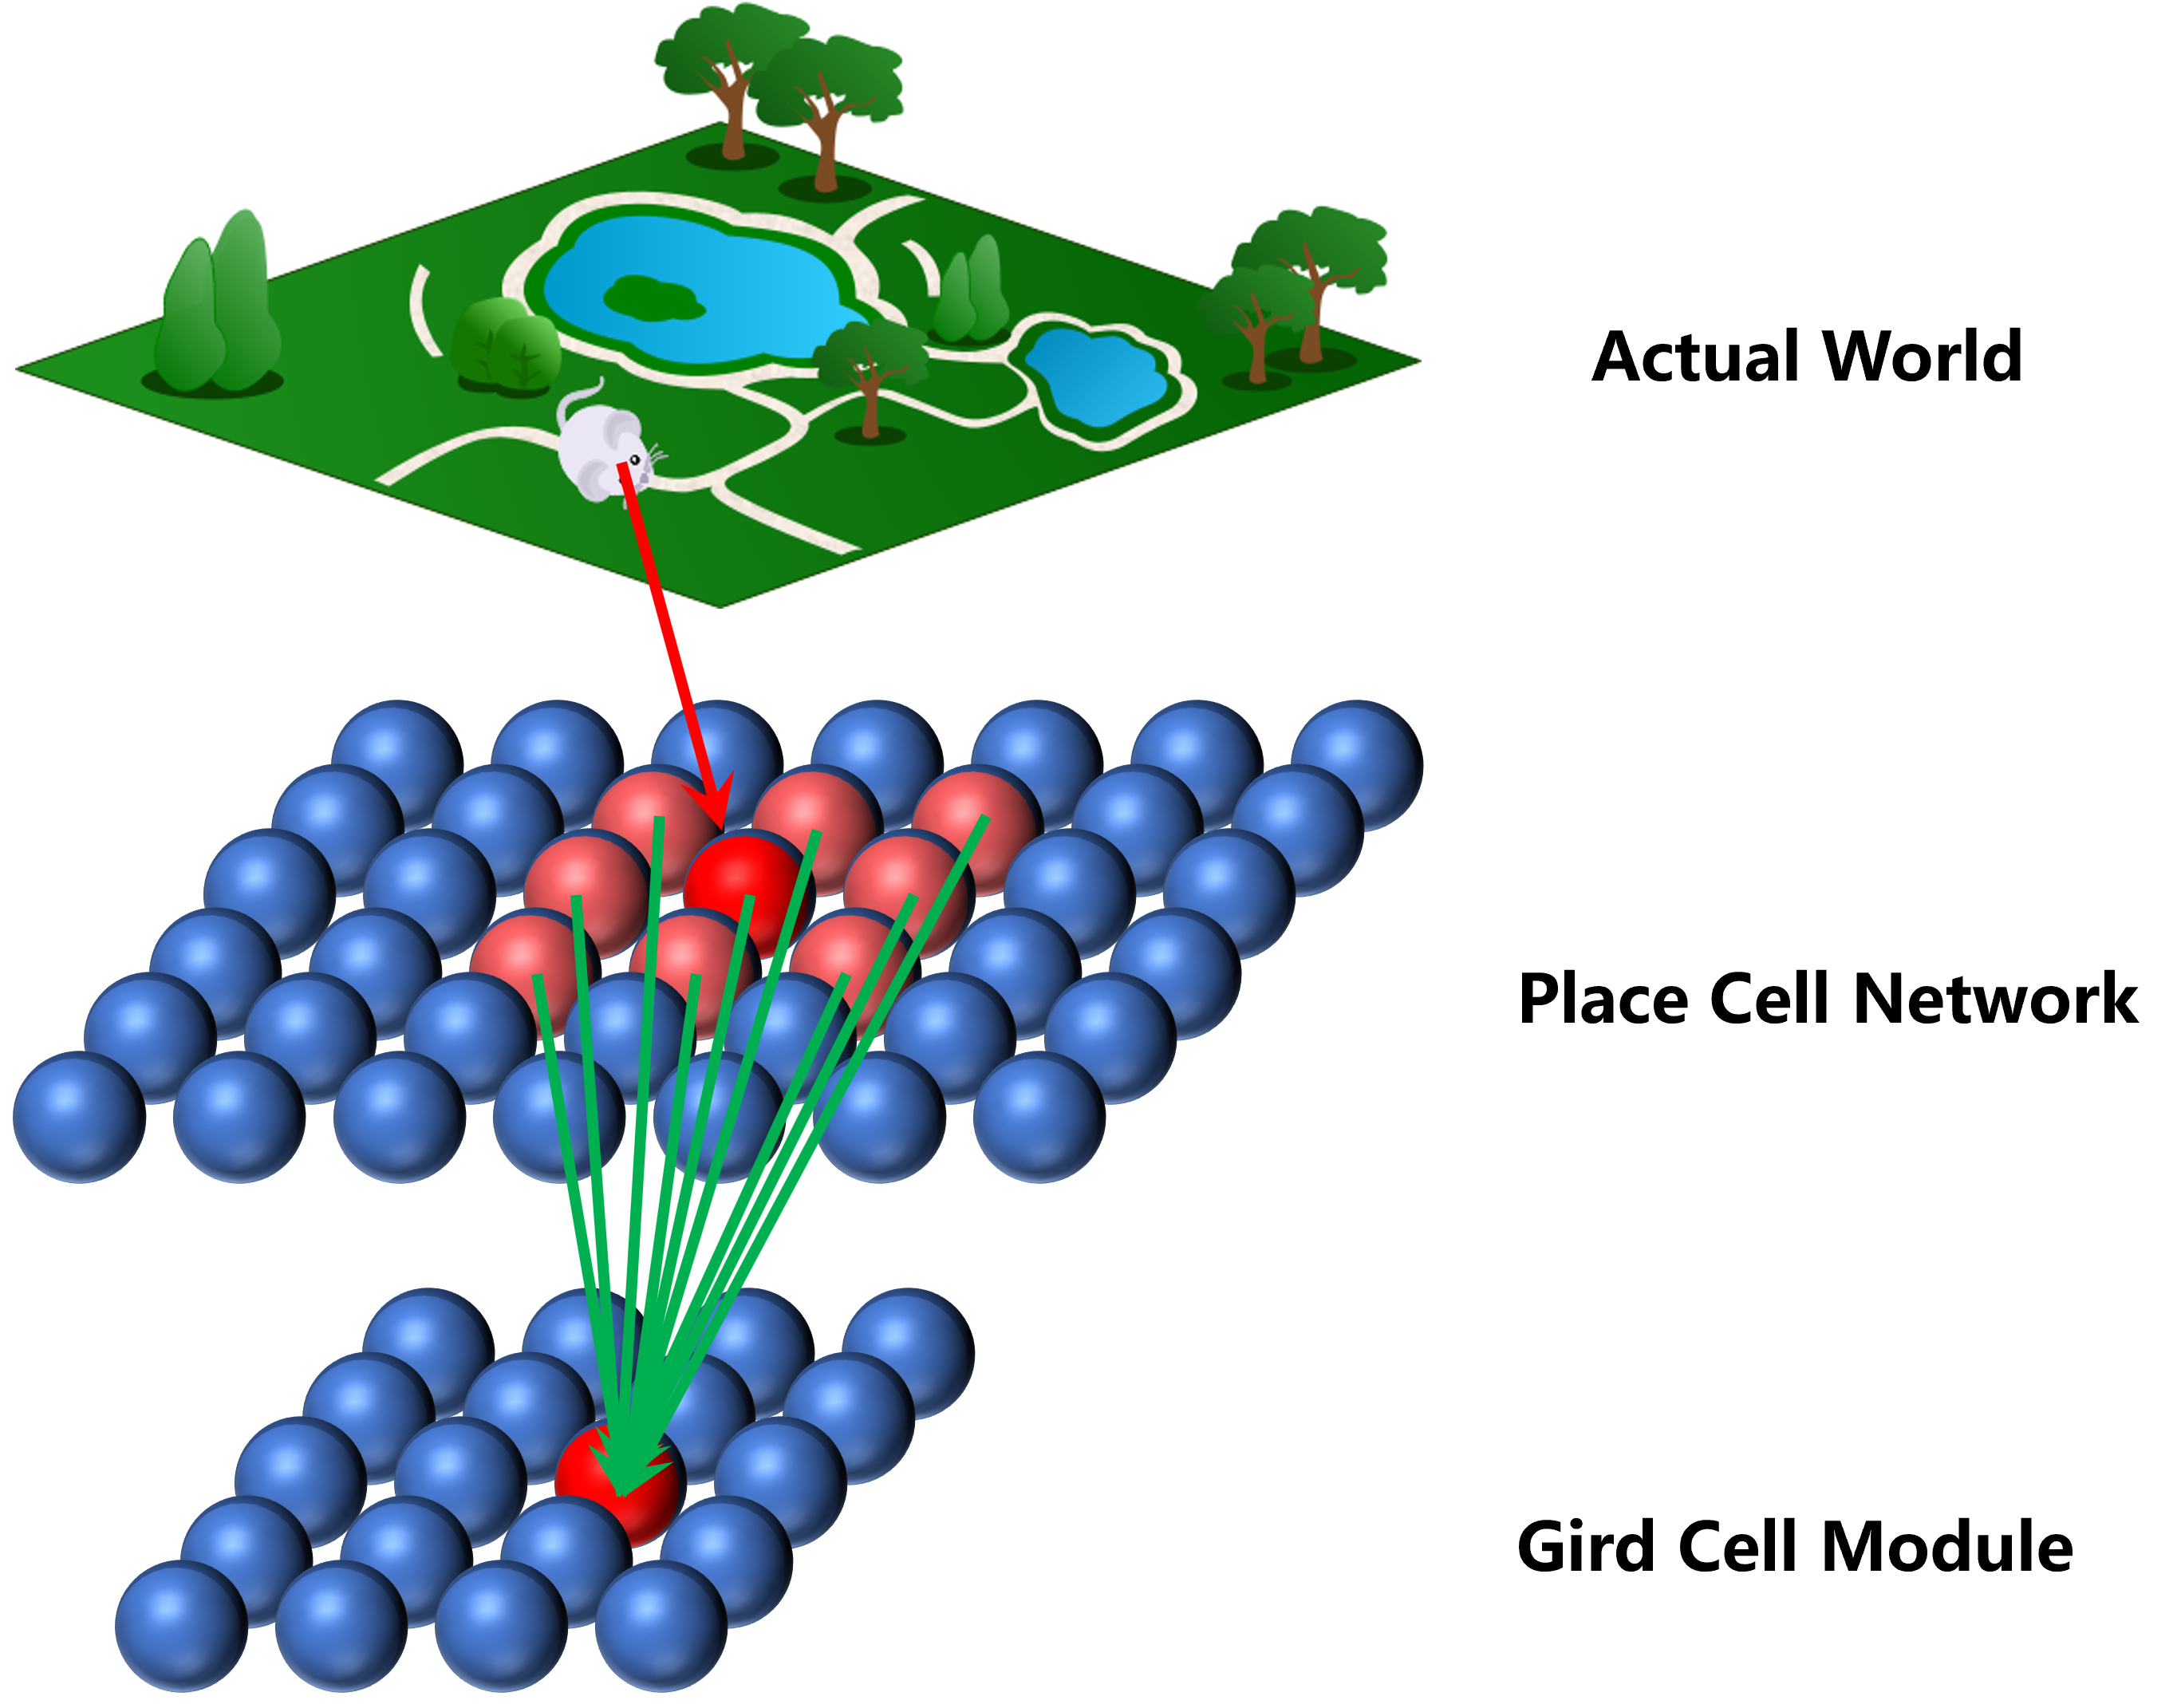
\includegraphics[width=0.9\linewidth]{Figure/w-p-g.png}
	\caption{The grid cell module receives excitation from external cues. In the top of the figure, the rat moves in the actual world. The place cell CANN network and grid cell module are driving by the velocity and the head direction from the speed cells and head direction cell of the rat. When the rat receive the excitation from landmark, the bump position of the place cell network will be used to activate the grid cell module by the Eq.~\eqref{eq:cal_rate} and Eq.~\eqref{eq:cal_position}.}
	\label{fig:w2p2g}
\end{figure*}

\begin{equation}\label{eq:worldframe2pcframe} 
	\boldsymbol{P^p_i} = \boldsymbol{R_{wp_i}}\cdot \boldsymbol{P^w_i} + \boldsymbol{\varpi_i}
\end{equation}	
where $\boldsymbol{R_{wp}}$ and $\boldsymbol{\varpi}$ are the rotation matrix and translation vector. And $\boldsymbol{R_{wp}}$ can be described by the rotation angle $\phi$ as follows:
\begin{equation}\label{eq:rotation_matrix}
	\boldsymbol{R_{wp}} =
	\begin{bmatrix}
		cos\phi& -sin\phi\\
		sin\phi& cos\phi
	\end{bmatrix}^{-1}
\end{equation}
This can inject energy for place cell CANN model. Then the excitation can be updated according to the weights between place cells neurons in the sheet\cite{McNaughton2006c}. After the process of competitive attractor network dynamics, the network of place cells gradually is stabilized. Then the neuron that have maximum firing rate is found and marked as $\boldsymbol{P^p_\text{max}}$. It will be transform into grid cells firing space by:
\begin{align}\label{eq:cal_position}
	\bm{P^g_i} &= \bm{R_{pg}}\cdot \bm{P^p_\text{max}} 
\end{align}
where $\boldsymbol{P^g_i}$ is the corresponding neuron position in the PhaseCANN, $\boldsymbol{R_{pg}}$ is the transformation matrix and it can be depicted as follows:
\begin{align}
	\boldsymbol{R_{pg}} =
	\begin{bmatrix}
		s\cdot cos(o_i)& s\cdot cos(o_i+\pi/3)\\
		s\cdot sin(o_i)& s\cdot sin(o_i+\pi/3)
	\end{bmatrix}^{-1}
\end{align}
where $s$ and $o$ separately is the spacing and orientation of the grid cell module. For the firing rate of $\bm{P^g_i}$, it can be calculated as follows:
\begin{equation}\label{eq:cal_rate}
	\varsigma_i = \sum_{k=1}^{M} \mathcal{T}_{ik} \mathcal{F}(\bm{P^p_k})
\end{equation}
where $\varsigma_i$ is the firing rate of $\bm{P^g_i}$, $M$ is the neural population of the place cell network, $\mathcal{T}_{ik}$ is the weight profile that is learned by Hebbian rule, $\mathcal{F}(\cdot)$ is the function to acquire the firing rate of $\bm{P^p_k}$ in the place cell network.

In this way, the PhaseCANN can acquire excitation from the external cues. So the firing rate of single neuron in the Eq.~\eqref{eq:firing_rate} can be further described as follows:
\begin{equation}\label{eq:firing_rate_modify}
	\tau \frac{d r_{i}}{d t}+r_{i}=f\left[\sum_{j} w_{i j} r_{j} + Q_i\right]
\end{equation}
where $Q_i$ is the feedforward input to neuron $i$ from external cues. After receiving the external excitation, the PhaseCANN need to process the excitatory update. A two-dimension discrete Gaussian distribution is used to generate the excitatory weight matrix, $w_{ij}$, which is depicted in Eq.~\eqref{eq:weight_gc}. Then each neuron uses it to project activity to all other neuron in the PhaseCANN.

Finally, the PhaseCANN is normalized to constrain the sum of activation in whole network. Before normalization, the firing rate of each neuron need to be maintained a scope by Heaviside function. Then the normalization process can be described as follows:
\begin{equation}\label{eq:normalization}
	\tilde{\varsigma_i} = \frac{\varsigma_i}{\sum_{j=1}^{N} \varsigma_j}
\end{equation}
where $\tilde{\varsigma_i}$ is the firing rate after normalization, $N$ is the neuron population of PhaseCANN.

% TODO: \usepackage{graphicx} required


To verify the ability of receiving the excitation of the network, a PhaseCANN was established according to \ref{subsection:structure} and \ref{subsection:connection}. The parameters of the network mentioned are listed in Tab.\ref{tab:model_parameter}.

\begin{table}[h]
	\centering
	\caption{The parameters of the PhaseCANN}
	\label{tab:model_parameter}
	\begin{tabular}{c c c c c c c c c }		
		\toprule
		\textbf{Parameters}&$N_x$& $N_y$&$s$ &$o$ &$\alpha$ &$\beta$ &$\rho$ &$gamma$ \\
		\midrule
		\textbf{value}&100&100&1.0&$\pi/3$&1.0&1.0&0.01&0.003\\
		\bottomrule
	\end{tabular}
\end{table}

As the Fig.~\ref{fig:show_excitation} depicted, multiple position was injected energy and the activity bump was formed by diffusing the excitation using the connection between neurons. In addition, latter position injected energy inhibited the former. For this reason, the former positions remain a dim bump in Fig.~\ref{fig:show_excitation_b}-\ref{fig:show_excitation_d}.
In addition, comparing the Fig.~\ref{fig:show_excitation_b} and Fig.~\ref{fig:show_excitation_c}, the previous bump in center position will be disappeared with injecting energy in new position. This demonstrates that our model have suitable weight connection between neurons to perform excitation and inhibition. When the bump position is in the edge of network sheet, the bump will appear in the opposite edge of the sheet depicted in Fig.~\ref{fig:show_excitation_c} and Fig.~\ref{fig:show_excitation_d}. This demonstrate the our model exist the periodic boundary condition.

\begin{figure*}[!t]
	\subfigcapskip=-10pt %调整子图片与子标题的距离
	\centering
	\subfigure[]{
		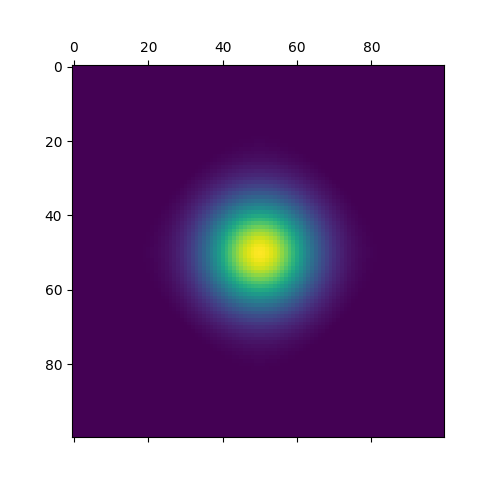
\includegraphics[width=0.25\linewidth]{Figure/show_excitation_1.png}
		%\caption{fig1}
		\label{fig:show_excitation_a}
	}
	\hspace{-8mm}
	\subfigure[]{
		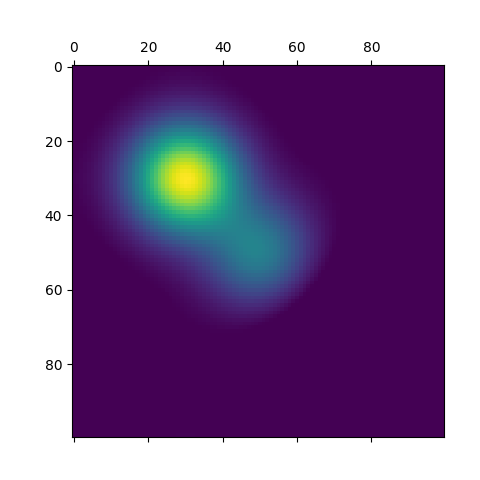
\includegraphics[width=0.25\linewidth]{Figure/show_excitation_2.png}
		\label{fig:show_excitation_b}
	}
	\hspace{-8mm}
	\subfigure[]{
		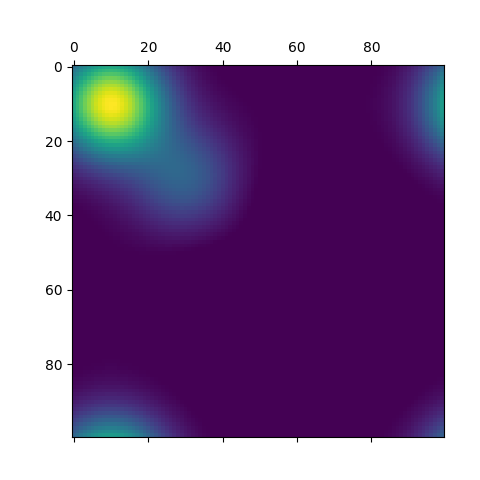
\includegraphics[width=0.25\linewidth]{Figure/show_excitation_3.png}
		\label{fig:show_excitation_c}
	}
	\hspace{-8mm}
	\subfigure[]{
		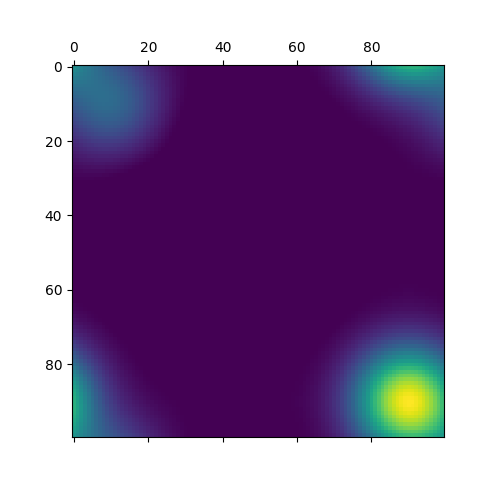
\includegraphics[width=0.25\linewidth]{Figure/show_excitation_4.png}
		\label{fig:show_excitation_d}
	}
	\caption{Activity and stabilization. The yellow color and blue color represent the high and low excitatory region separately. (a)Firstly, the network is injected energy in $(50,50)$. Then the energy is spread by synaptic weight profile and the activity bump is formed in the sheet. (b). After that, the network is injected in new position $(30,30)$. Then the internal dynamic is performed to stabilize whole network. The new excitatory region appear a highest bump and previous excitatory region remain a lower bump. (c) Similar to (b), the network is injected energy in $(10,10)$. (d)Similar to (b), the network is injected energy in $(90,90)$. Because of the periodic boundary, the excitatory bump appear in four corner of the network.}
	\label{fig:show_excitation}
\end{figure*}

\subsection{Path integration}

For the CANN models, the path integration is a important ability comparing with other models of grid cells. The path integration process updates the network activity by shifting the activated bump based on the velocities and head direction angles from speed cell\cite{Kropff2015} and head direction cell\cite{Zhang1996,Taube1990}. In general, the path integration in CANN models is performed by projecting existing neural bump to the future location and dynamically shifting the current activity to towards the future location. Another method of the path integration shifting existing neural bump rather than projecting a copy of the current activity. This approach makes the performance of the robot independent of varying sensory update rates and robot velocity, resulting in more precise robot trajectories and eliminating the need for parameter adjustment\cite{Milford2008d}. In here, the latter method was chosen to process the path integration. However, different with \cite{Milford2008d}, in here, the translation in the world frame needs to be transformed into PhaseCANN and the computation of firing rate is performed using the convolution kernel.

After the rat move a distance per unit time, the offsets can be calculated as follows:
\begin{equation}\label{eq:offsets}
	\begin{aligned}
		\Delta x^w_i &= \int_{t_{i}}^{t_{i+1}}|\bm{v}(t)| \cdot cos\alpha(t) \ \text{d}t	\\
		\Delta y^w_i &= \int_{t_{i}}^{t_{i+1}}|\bm{v}(t)| \cdot sin\alpha(t) \ \text{d}t
	\end{aligned}
\end{equation}

where $\Delta x^w_i$ and $\Delta y^w_i$ are the translation of two directions in the world frame, $\bm{v}(t)$ and $\alpha(t)$ are the translation velocity and head direction separately.

Then the translation in the world frame can be transformed into PhaseCANN by:
\begin{align}\label{eq:trans_w2g}	
	[\Delta x^g_i,\Delta y^g_i]^T &= \bm{R_{pg}}\cdot \bm{R_{wp}} [\Delta x^w_i,\Delta y^w_i]^T 
\end{align}
where $\Delta x^g_i$ and $\Delta y^g_i$ are the offsets in the PhaseCANN.

For a neuron $\epsilon_{xy}$ in $(x,y)$ of the PhaseCANN, its firing rate $\varsigma_{xy}$ can be update by the path integration as follows:
\begin{equation}\label{rate_path_integration}
	\varsigma_{xy}' = \sum_{a=\delta x_o }^{\delta x_o +1}\sum_{b=\delta y_o}^{\delta y_o +1} \eta_{ab} \varsigma_{(x+a)(y+b)}
\end{equation}
where $\eta_{ab}$ is a $2\times2$ convolution kernel to compute the firing rate of $\varsigma_{xy}$. Every item of $\eta_{ab}$ can be acquired as follows:
\begin{equation}\label{convolution_kernel}
	\eta_{ab} = \frac{\sqrt{(a-\Delta x_i^g)^2+(b-\Delta y_i^g)^2}}{\sum_{a=\delta x_o }^{\delta x_o +1}\sum_{b=\delta y_o}^{\delta y_o +1}\sqrt{(a-\Delta x_i^g)^2+(b-\Delta y_i^g)^2}}
\end{equation}
where $\delta x_o,\delta y_o $ are the rounded down integer offsets in the $x$ and $y$ directions of the PhaseCANN, they can be calculate as follows:
\begin{equation}\label{rounded-offsets}
	\begin{bmatrix}
		\delta x_o\\
		\delta y_o
	\end{bmatrix}
	= 	
	\begin{bmatrix}
		\lfloor \Delta x_i^g \rfloor\\
		\lfloor \Delta y_i^g \rfloor
	\end{bmatrix}
\end{equation}
where $\lfloor \cdot \rfloor$ represents the rounded operation.

A virtual path is generated in a $5\times5$ square virtual environment to simulate the animal's path. During this process, the velocity and angle of the virtual point was recorded and used to drive the proposed network. The properties of grid cell module are similar to Table.\ref{tab:model_parameter}. In addition, the world frame and the frame of place cell firing space are set up identically. In other words, the rotation matrix $\bm{R_{wp}}$ is the identity matrix and the translation vector $\boldsymbol{\varpi}$ is the zero vector. 

\begin{figure*}[!t]
	\subfigcapskip=-10pt %调整子图片与子标题的距离
	\centering
	\subfigure[]{
		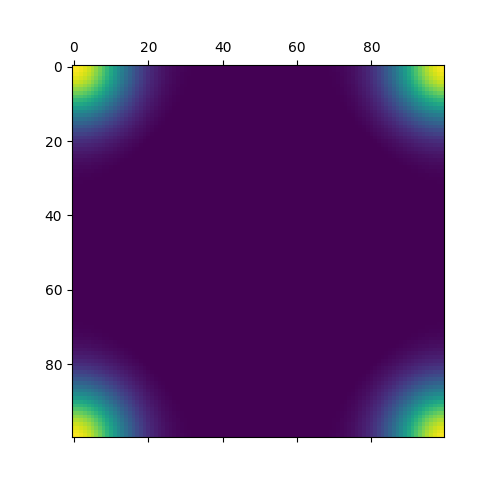
\includegraphics[width=0.2\linewidth]{Figure/drive_bump_1.png}
		%\caption{fig1}
		\label{fig:drive_bump_a}
	}
	\hspace{-8mm}
	\subfigure[]{
		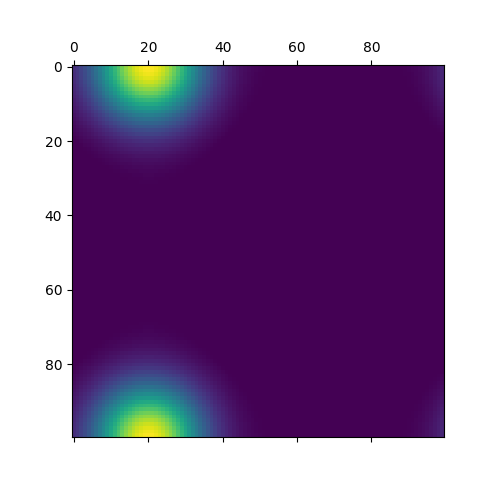
\includegraphics[width=0.2\linewidth]{Figure/drive_bump_3.png}
		\label{fig:drive_bump_b}
	}
	\hspace{-8mm}
	\subfigure[]{
		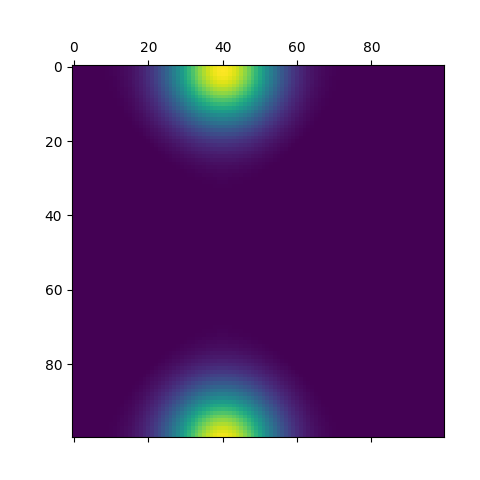
\includegraphics[width=0.2\linewidth]{Figure/drive_bump_5.png}
		\label{fig:drive_bump_c}
	}
	\hspace{-8mm}
	\subfigure[]{
		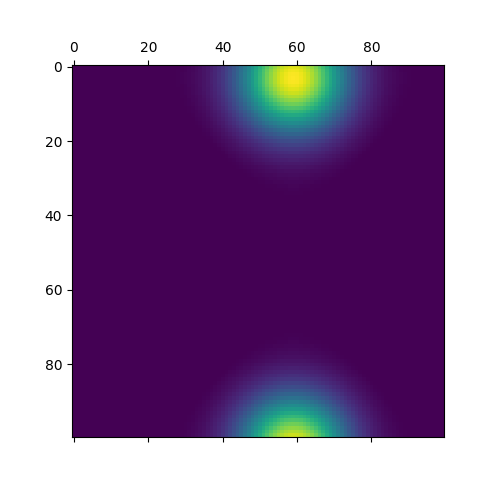
\includegraphics[width=0.2\linewidth]{Figure/drive_bump_7.png}
		\label{fig:drive_bump_d}
	}
	\hspace{-8mm}
	\subfigure[]{
		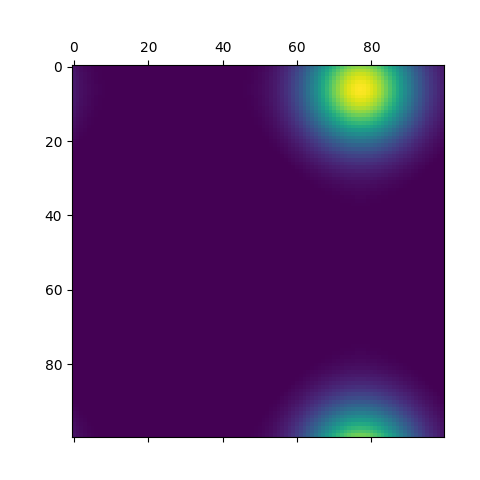
\includegraphics[width=0.2\linewidth]{Figure/drive_bump_9.png}
		\label{fig:drive_bump_e}
	}
	
	\vspace{-10pt}
	\subfigure[]{
		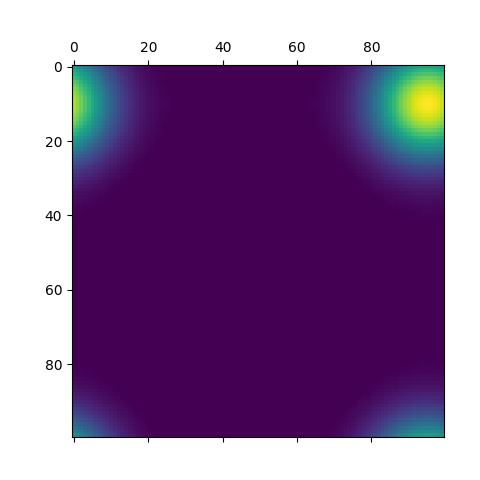
\includegraphics[width=0.2\linewidth]{Figure/drive_bump_11.png}
		%\caption{fig1}
		\label{fig:drive_bump_f}
	}
	\hspace{-8mm}
	\subfigure[]{
		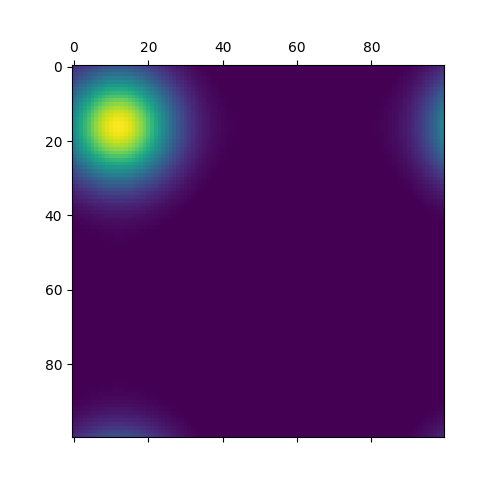
\includegraphics[width=0.2\linewidth]{Figure/drive_bump_13.png}
		\label{fig:show_excitation_g}
	}
	\hspace{-8mm}
	\subfigure[]{
		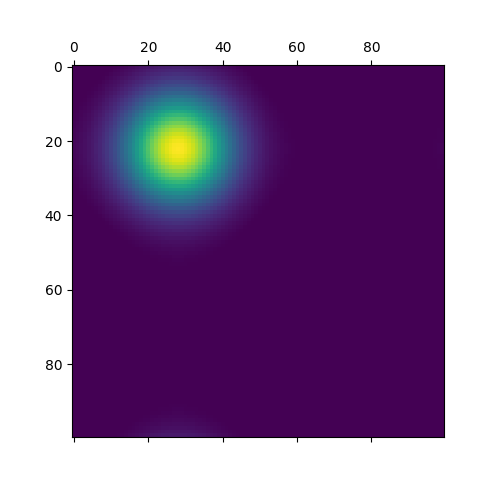
\includegraphics[width=0.2\linewidth]{Figure/drive_bump_15.png}
		\label{fig:drive_bump_h}
	}
	\hspace{-8mm}
	\subfigure[]{
		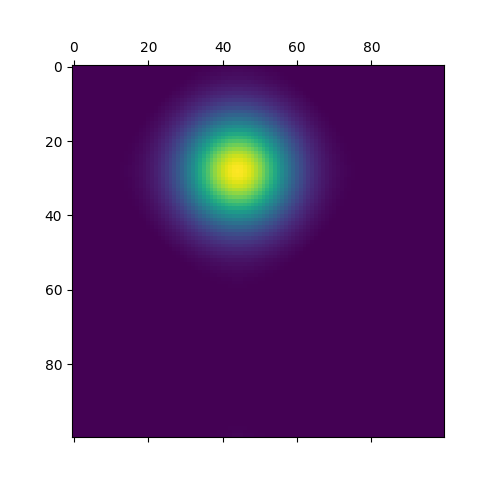
\includegraphics[width=0.2\linewidth]{Figure/drive_bump_17.png}
		\label{fig:drive_bump_i}
	}
	\hspace{-8mm}
	\subfigure[]{
		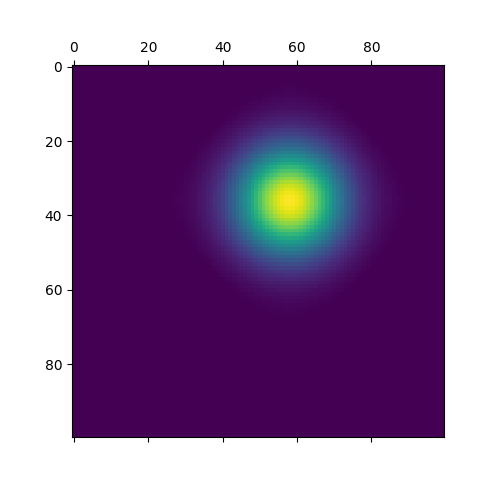
\includegraphics[width=0.2\linewidth]{Figure/drive_bump_19.png}
		\label{fig:drive_bump_j}
	}
	\caption{The snapshots of network status during the path integration. In the figure, different colors represent different firing rates of the neurons. The firing rates gradually decline through yellow to blue. In the beginning, as the (a) shown, the origin point is the $(0,0)$ and so the corresponding neuron in the $(0,0)$ is activated. Along the moving of virtual point in the environment, the excitatory bump begin to move. In addition, the snapshots are chosen per two time steps in here to better show the process.}
	\label{fig:drive_bump}
\end{figure*}

In per time step, the offsets are calculated by Eq.~\eqref{eq:offsets}. Then the firing rate of every neuron in the PhaseCANN can be updated by Eq.~\eqref{eq:trans_w2g}-\eqref{rounded-offsets}. The several snapshots of the network status during this process are depicted in Fig.~\ref{fig:drive_bump}. The excitatory bump continuously move in the network sheet. This demonstrates PhaseCANN can maintain the stability and perform the path integration. When the bump reach to the edges of the network sheet depicted in the Fig.~\ref{fig:drive_bump_e} and Fig.~\ref{fig:drive_bump_f},the bump will appear in opposite edge because of the periodic boundary condition.

To show the activity of single grid cell in the module, three neurons in the network are chosen to record their activity during the path integration. In addition, the parameters of network set up are similar to the  Table.\ref{tab:model_parameter}. But the spacing of grid cell module is set to $1.20$ in here. When the bump move through these neurons, the neurons acquire excitatory condition. By this way, the firing patterns of single grid cell are recorded depicted in the Fig.~\ref{fig:single_neuron_firing}. The Figure shows that the firing patterns of single grid cell approximately are hexagonal. This is consistent with the properties of grid cells and experiment results\cite{Hafting2005}.

\begin{figure*}[!t]
	\subfigcapskip=-10pt %调整子图片与子标题的距离
	\centering
	\subfigure[]{
		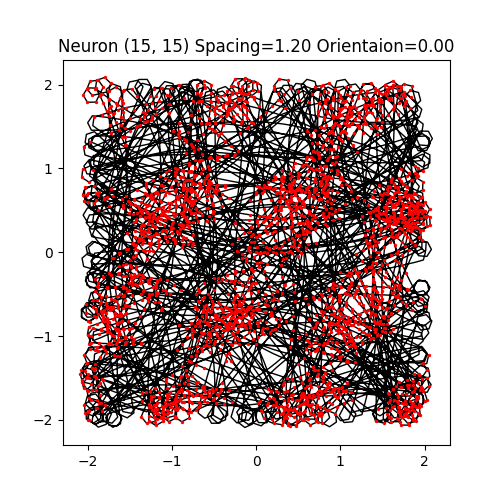
\includegraphics[width=0.33\linewidth]{Figure/single_neuron_firing_1.png}
		%\caption{fig1}
		\label{fig:single_neuron_firing_a}
	}
	\hspace{-8mm}
	\subfigure[]{
		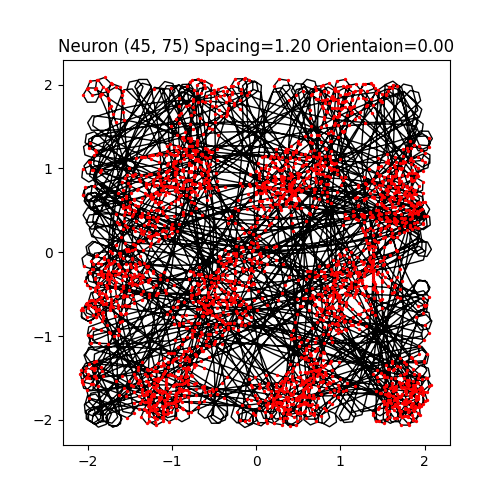
\includegraphics[width=0.33\linewidth]{Figure/single_neuron_firing_2.png}
		\label{fig:single_neuron_firing_b}		
	}
	\hspace{-8mm}
	\subfigure[]{
		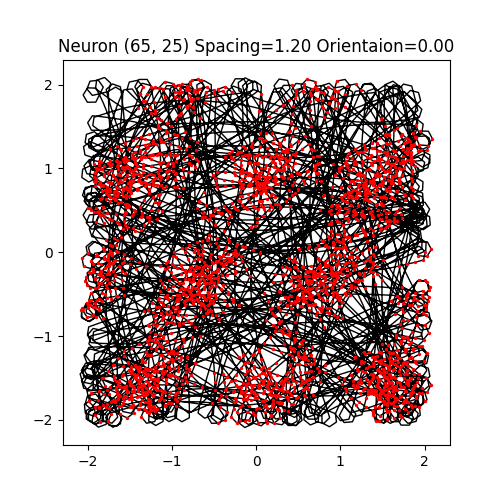
\includegraphics[width=0.33\linewidth]{Figure/single_neuron_firing_3.png}
		\label{fig:single_neuron_firing_c}		
	}
	\caption{The firing patterns of the single grid cell in the different position of the PhaseCANN. The black lines in the three figures are the paths that are generated in the virtual environment. The red points represents the firing condition of single neuron. (a) The firing pattern of the neuron in the position $(15,15)$ of the network. (b) The firing pattern of the neuron in the position $(45,75)$ of the network. (c) The firing pattern of the neuron in the position $(65,25)$ of the network.}
	\label{fig:single_neuron_firing}
\end{figure*}

To further demonstrate the activities of single neuron in different grid cell module, we establish nine PhaseCANN with different spacing and orientation. Then the firing activities in same position of these networks are recorded with driving the networks using the moving path mentioned above. The results are shown in Fig.~\ref{fig:single_neuron_firing_diff_prop}. Comparing the figures from left to right, the firing patterns are rotated with increasing orientation of the grid cell. In addition, the change of interval is consistent with the increasing spacing of the grid cell module. This demonstrates our proposed model can be applied in different properties of grid cells. In previous researches\cite{Bush2015,Edvardsen2020}, the gird-like patterns are used as accurate path integration. In here, the grid-like patterns are generated. But the patterns are obviously irregular and snatchy. Although the patterns generated are consistent with the observation of the biological experiment\cite{Hafting2005}, they are hard to use as a accurate path integration. According to our concept, path integration should be performed using a single grid cell module rather than a single grid cell.


\begin{figure*}[!t]
	\vspace{-2pt}
	\subfigcapskip=-10pt %调整子图片与子标题的距离
	\centering
	\subfigure[]{
		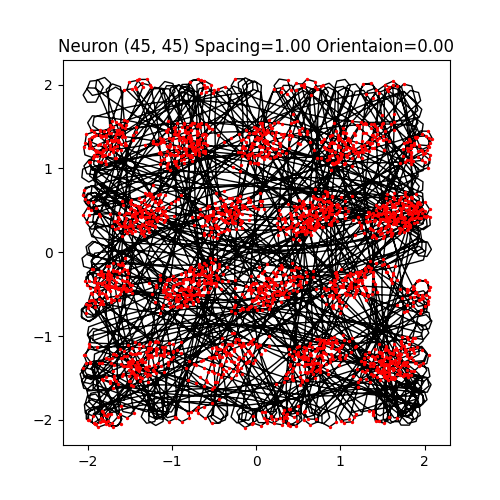
\includegraphics[width=0.33\linewidth]{Figure/single_neuron_firing_1.0_0.00.png}
		%\caption{fig1}
		\label{fig:single_neuron_firing_diff_prop_a}
	}
	\hspace{-8mm}
	\subfigure[]{
		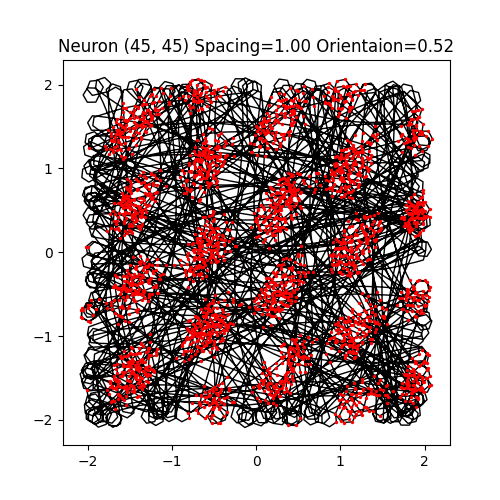
\includegraphics[width=0.33\linewidth]{Figure/single_neuron_firing_1.0_0.52.png}
		\label{fig:single_neuron_firing_diff_prop_b}		
	}
	\hspace{-8mm}
	\subfigure[]{
		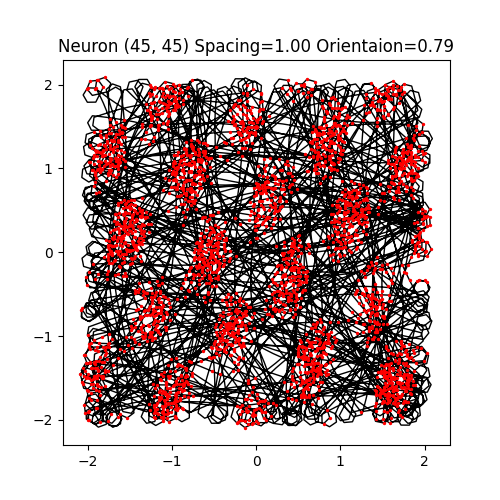
\includegraphics[width=0.33\linewidth]{Figure/single_neuron_firing_1.0_0.79.png}
		\label{fig:single_neuron_firing_diff_prop_c}		
	}


\vspace{-10pt}
	\subfigure[]{
	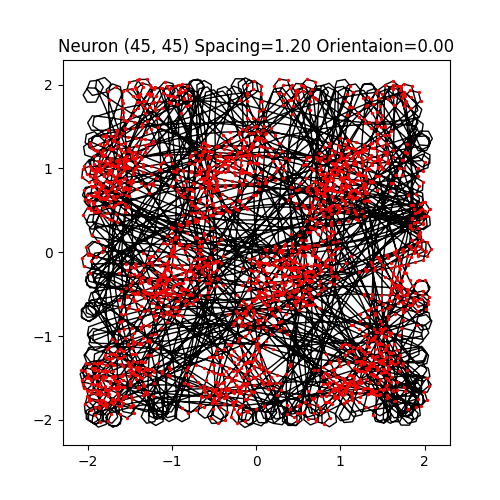
\includegraphics[width=0.33\linewidth]{Figure/single_neuron_firing_1.2_0.00.png}
	%\caption{fig1}
	\label{fig:single_neuron_firing_diff_prop_d}
}
\hspace{-8mm}
\subfigure[]{
	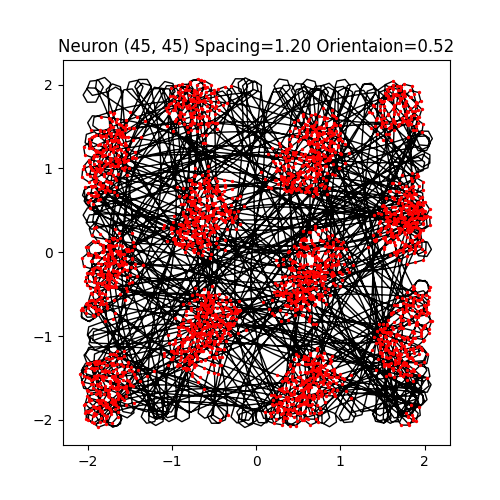
\includegraphics[width=0.33\linewidth]{Figure/single_neuron_firing_1.2_0.52.png}
	\label{fig:single_neuron_firing_diff_prop_e}		
}
\hspace{-8mm}
\subfigure[]{
	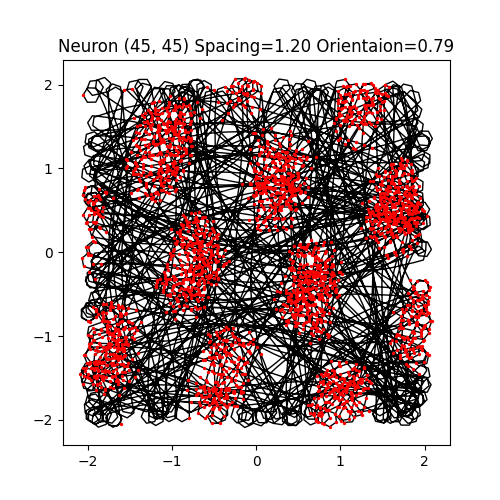
\includegraphics[width=0.33\linewidth]{Figure/single_neuron_firing_1.2_0.79.png}
	\label{fig:single_neuron_firing_diff_prop_f}		
}

\vspace{-10pt}
	\subfigure[]{
	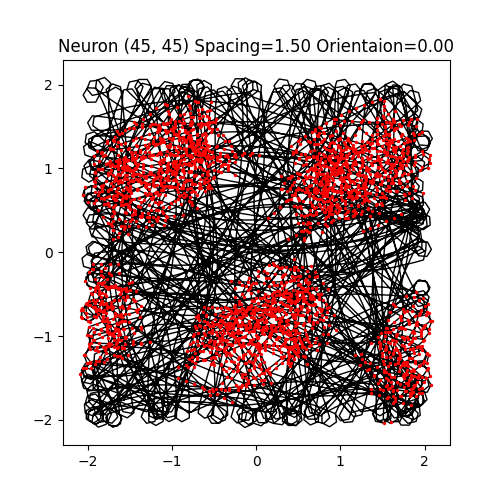
\includegraphics[width=0.33\linewidth]{Figure/single_neuron_firing_1.5_0.00.png}
	%\caption{fig1}
	\label{fig:single_neuron_firing_diff_prop_g}
}
\hspace{-8mm}
\subfigure[]{
	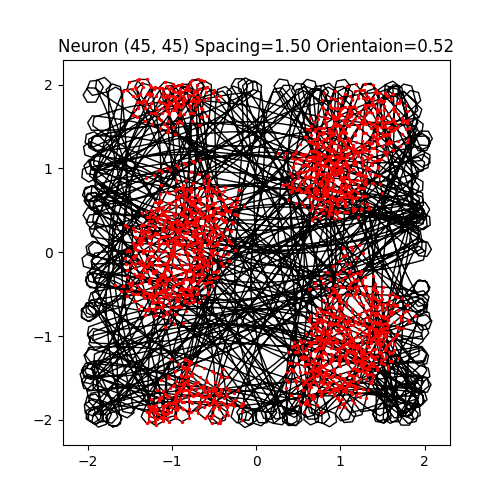
\includegraphics[width=0.33\linewidth]{Figure/single_neuron_firing_1.5_0.52.png}
	\label{fig:single_neuron_firing_diff_prop_h}		
}
\hspace{-8mm}
\subfigure[]{
	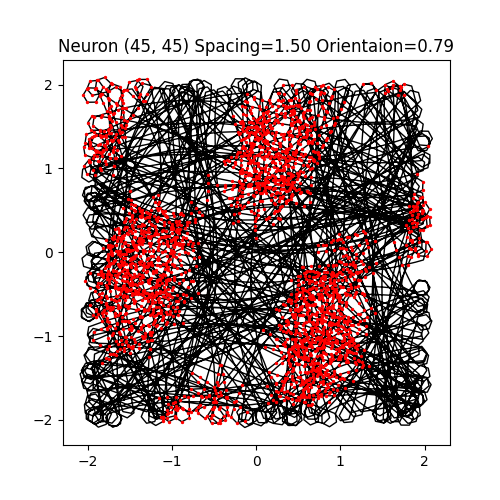
\includegraphics[width=0.33\linewidth]{Figure/single_neuron_firing_1.5_0.79.png}
	\label{fig:single_neuron_firing_diff_prop_i}		
}
	\caption{The firing patterns of the single grid cell in the different module but in same position of the PhaseCANN. }
	\label{fig:single_neuron_firing_diff_prop}
	\vspace{-2pt}
\end{figure*}


To verify the ability of our model to perform path integration, several experiments are designed. We compare the performance of different PhaseCANN models that have different spacing of grid cell and different size of network in the Eq.~\eqref{eq:network_size}. The results of experiment are shown in Fig.~\ref{fig:path_integration}. In general, the error of path integration gradually increases with moving steps. For different spacing of grid cells, the error of bigger spacing is more obvious than the smaller in Fig.~\ref{fig:path_integration_a}. In addition, the size of network also influence the 
deviation of path integration. The more neurons in the network can acquire the lower error of path integration in general. In here, the precise $\mathcal{J}$of path integration can be described as follows:
\begin{equation}\label{eq:relation_precise}
	\mathcal{J} \varpropto \frac{1}{s/N} = \frac{1}{\varrho}
\end{equation}
where $s$ represents the spacing of grid cells, $N$ is the size of the network, $\varrho$ is the ratio of $s$ and $N$ marked as network resolution ratio of CANN. According to the results of experiment depicted in Fig.~\ref{fig:path_integration}, we infer that the precise of path integration is proportional to the network resolution ratio $\varrho$. 

\begin{figure*}[!t]
%	\subfigcapskip=-10pt %调整子图片与子标题的距离
	\centering
	\subfigure[]{
		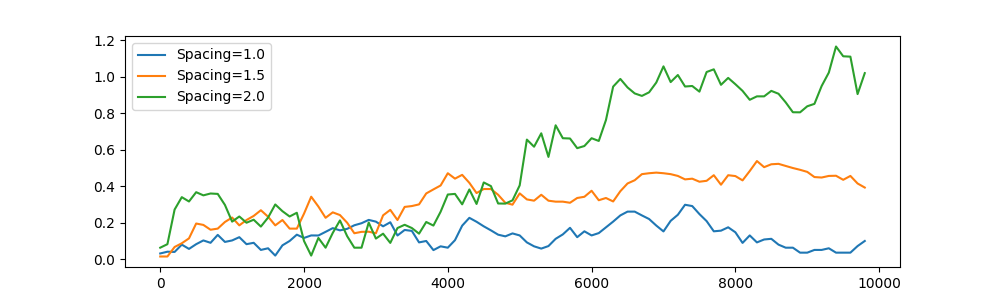
\includegraphics[width=0.9\linewidth]{Figure/diff_spacing.png}
		%\caption{fig1}
		\label{fig:path_integration_a}
	}

	\vspace{-10pt}
	\subfigure[]{
		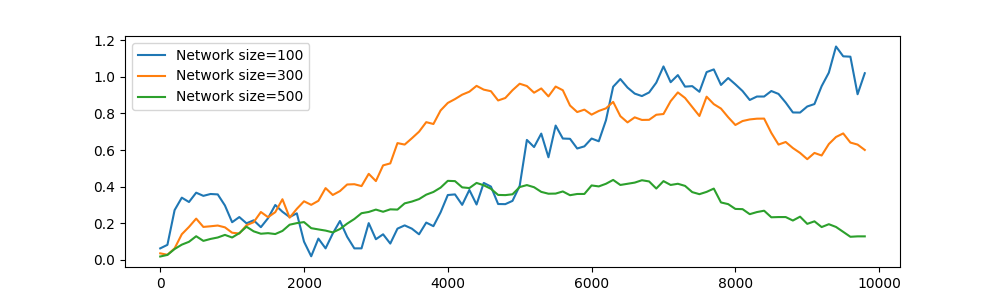
\includegraphics[width=0.9\linewidth]{Figure/diff_netsize.png}
		\label{fig:path_integration_b}		
	}
	
	\caption{The error of path integration using PhaseCANN with iterations. The x-axis is the moving steps. (a) The error of path integration using different spacing in the PhaseCANN but same size of network, i.e., $100$. (b) The error of path integration using different network sizes in the PhaseCANN but same spacing of grid cell, i.e., $2.0$. }
	\label{fig:path_integration}
\end{figure*}

In general, the error of path integration is accumulated with iteration. To eliminate the error, the visual cues are introduced and correct the deviation. In our model, as Fig.~\ref{fig:w2p2g} shown, the landmarks in the actual world are mapping to the network of place cells. Then the excitation in the place cell network is transformed and mapping to the firing space of grid cells. This can help the grid cell module to reduce the influence from accumulative error. In here, the excitation from place cell are injected into network of the grid cell module per $500$ steps. The error of path integration is recorded per $100$ steps to obviously show the difference between PhaseCANN model with and without feedback. This comparison is shown in Fig.~\ref{fig:path_integration_feedback}. during the initial process, their error all remains a low level. However, along the increasing steps, the PhaseCANN with feedback still can keep a low deviation. In contrast, the error of the PhaseCANN without feedback will increasingly increase.  The results manifest our model have the ability to reduce the accumulated error.

\begin{figure*}[!t]
	%	\subfigcapskip=-10pt %调整子图片与子标题的距离
	\centering
	\subfigure{
		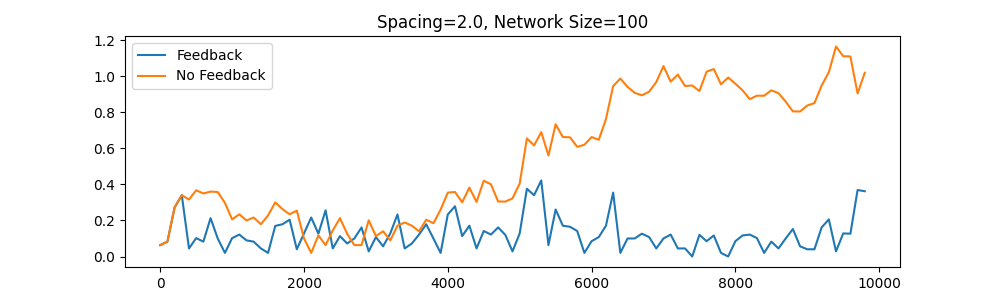
\includegraphics[width=1.0\linewidth]{Figure/PI_feedback.png}
		%\caption{fig1}		
	}
	\caption{Error comparison of path integration with and without feedback from a place cell network.  }
	\label{fig:path_integration_feedback}
\end{figure*}


\section{Discussion}
The rodent animals have outstanding navigation ability\cite{Ball2013}. They can walk a long way and return their dens. This demonstrates they have the splendid ability of path integration. However, the reason still be mysterious. The grid cells have draw enormous attention because of their properties. Specially, the periodic firing patterns of grid cells in the MEC can provide a compact  code for location within large-scale space\cite{Bush2015}. In addition, The general consensus is that grid cells provide a path integration input for place cells\cite{McNaughton2006}. In here, our model is used to perform the path integration in longer steps. This is depicted in Fig.~\ref{fig:path_integration_long}. In three different grid-cell modules, their error remains a scope even after $100000$ steps without feedback from place cells. This also can partly explains why the rodent animals can return their dens even though they have go for a very long distance. 
\begin{figure*}[!t]
	%	\subfigcapskip=-10pt %调整子图片与子标题的距离
	\centering
	\subfigure{
		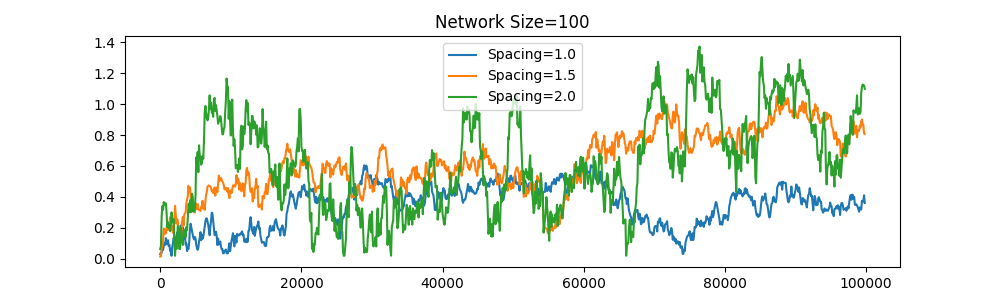
\includegraphics[width=1.0\linewidth]{Figure/PI_long.png}
		%\caption{fig1}		
	}
	\caption{Error comparison of path integration with and without feedback from a place cell network.  }
	\label{fig:path_integration_long}
\end{figure*}

In summary, the PhaseCANN model was proposed for grid-cell module. Then the self-motion inputs are designed to drive the PhaseCANN model. In addition, to provides visual feedback for grid-cell module during the process of the path integration, the connection between place cell and grid cell is established. Simultaneously, the hexagonal firing patterns of single grid cell can be acquired by recording the firing activity of single neuron in the PhaseCANN model. Finally, we use our model to perform the path integration and comparing the results in different grid-cell properties and sizes of the PhaseCANN. The results point out that the network resolution ratio can influence the accuracy of the path integration. Furthermore, the results also manifests that our model can acquire outstanding performance even in the absence of external cues and on a large scale.
\section{Declaration of Competing Interest}
The authors declare that they have no known competing financial interests or personal relationships that could have appeared to influence the work reported in this paper.
\section{Acknowledgments}

%% If you have bibdatabase file and want bibtex to generate the
%% bibitems, please use
%%
 \bibliographystyle{elsarticle-num} 
 \bibliography{zotero}

%% else use the following coding to input the bibitems directly in the
%% TeX file.

% \begin{thebibliography}{00}

% %% \bibitem{label}
% %% Text of bibliographic item

% \bibitem{}

% \end{thebibliography}
\end{document}
\endinput
%%
%% End of file `elsarticle-template-num.tex'.
